This group design project was focused on building a downwind faster than the wind (DWFTTW) vehicle. This concept designates a vehicle that can travel dead-downwind at greater-than-wind speeds relying solely on wind power. Starting from stationary, the wind accelerates the vehicle as a bluff body, turning its wheels. A propeller mechanically connected to the wheels rotates as the wheels turn, converting torque from the wheels into thrust. As the vehicle approaches wind speed, the propeller generates thrust even though the relative incoming airflow is almost zero, continuing to accelerate the vehicle above wind speed and beyond. The theoretical aspects of this concept are detailed in the "DWFTTW Working Principle" section. Although the functioning of this vehicle is unintuitive, it has been proven to work on numerous occasions, both in a real-world setting \cite{veritasiumvid} and in theory \cite{drela20dead}.

\subsection{Project Inspiration}

The major inspiration for this project came from Rick Cavallaro and John Borton's DWFTTW vehicle Blackbird, which recently acquired media attention from Derek Muller's YouTube channel Veritasium \cite{veritasiumvid}. Demonstrating the vehicle on the Ivanpah dry lake bed, south of Las Vegas, they achieved almost three times wind speed \cite{downwindRecord}. Despite numerous demonstrations of DWFTTW vehicles beating wind speed, scepticism among the scientific community exists to this day, with the commonly held belief that a vehicle with faster-than-wind capabilities would be a perpetual motion device, violating the first law of thermodynamics. One way to tackle this scepticism is to increase awareness of these vehicles, by building and demonstrating additional working prototypes backed by the scientific rigour of wind tunnel testing.

\subsection{Previous Attempts at Downwind-Faster-Than-The-Wind Vehicles}

Although the BlackBird is the main and best known full scale attempt at realising the concept of DWFTTW vehicles, it was not the first attempt at realising the concept. An engineer by the name of Andrew B. Bauer demonstrated, in 1969, what is believed to be the first instance of a real world operation of the concept. He also discussed DWFTTW vehicles and their workings in \cite{bauer1969faster}.

After bringing the concept back into the spotlight, Rick Cavallaro, with the help of James Borton, went on to build a full-scale, manned, vehicle. From this project sponsored by Google was born the BlackBird as shown in Figure \ref{fig:blackbird} \cite{nast_2022}. Starting in 2009, and after a year of development, they demonstrated the vehicle on the Ivanpah dry lake bed and achieved wind speeds of up to 2.5 times the wind \cite{barry_2010}. In a video published on YouTube, Rick Cavallaro also demonstrated that his vehicle was also able to operate as an UWFTTW vehicle \cite{upwindyoutube}.

\begin{figure}[!htbp]
    \centering
    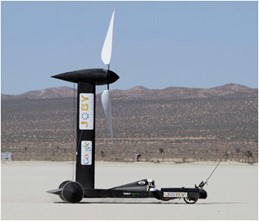
\includegraphics[width=0.6\linewidth]{images/part1/exisitingVeh3.jpg}
    \caption{The BlackBird by Rick Cavallaro and James Borton.}
    \label{fig:blackbird}
\end{figure}

\subsection{Upwind faster than the wind}

It is important to preface this section with the following: while reviewing the literature and other material available for this project, it quickly became clear that it was available in extremely limited quantity. Most of the publications available on the matter (such as \cite{mastersbs} and \cite{shetan}) somewhat paraphrase what is described in \cite{drela20dead}. It was therefore decided to take a closer look at a brother-concept, namely Upwind Faster Than The Wind (UWFTTW) vehicles, from which to draw inspiration, during the design phase of this project. 

The main difference between both concepts lies in the component playing the role of extracting energy from the wind. In the case of an upwind faster than the wind vehicle, the rotor acts as a turbine. It draws energy from the wind and provides torque to the wheels. Therefore, the vehicle is able to accelerate upwind. Although the anatomies of prototype vehicles for both concepts are nearly perfectly identical, it is important to emphasize the distinction between both: A DWFTTW vehicle features a propeller, and an UWFTTW vehicle features a turbine.

The main source of information on UWFTTW vehicles came from the Racing Aeolus competition. It is an annual competition for upwind faster than the wind vehicles, where teams from around the globe compete to travel the fastest against the wind. The competition started in 2018 with teams demonstrating a range of single-driver designs \cite{raeolus}. Most vehicles had a similar anatomy: a turbine mounted above an aerodynamic main body as seen on Figure \ref{fig:chinook}.

\begin{figure}[h]
    \centering
    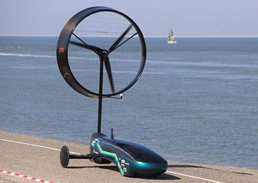
\includegraphics[width=0.6\linewidth]{images/part1/exisitingVeh2.png}
    \caption{Chinook 9, upwind faster than the wind prototype and winner of Racing Aeolus 2019 \cite{raeolus}.}
    \label{fig:chinook}
\end{figure}

In 2019 the fastest car (Figure \ref{fig:chinook}) achieved 114.8\% of the wind speed (which according to \cite{raeolus} was a world record at the time), and 114.0\% in 2018. This competition proves the possibility of achieving a velocity faster than the wind while going against it but also reinforces the difficulties of reaching this goal as the efforts of many of the previous teams in the Aeolus competitions demonstrate lower values than the wind speed. Taking inspiration from these vehicles facilitated early prototyping. 


